\chapter{Implementation}
\label{chapter:implementation}

The previous chapter elaborated on a redesign strategy addressing all of the identified issues that impair the usability of AMCS on mobile devices.
This chapter covers the realization of said changes in the form of a prototypical application. However, not all proposals were implemented as specified. One reason for this is that several problems arose during development such as legacy code that could not be changed easily without requiring a complete rewrite. The existing code base is complicated and hard to understand, as several different individuals worked on it over the years.
\\
\\ 
Another reason is some of the proposals themselves, as they were not thought through to the end or even deemed impractical without necessary improvements. Nevertheless, parts of the concept were adapted and a prototype was successfully implemented.
In the following, the implementation process and the required adjustments to the concept will be elaborated by describing different design iterations and the decisions behind each change.

\begin{figure}
	\centering
	\begin{minipage}[t]{.5\textwidth}
		\centering
		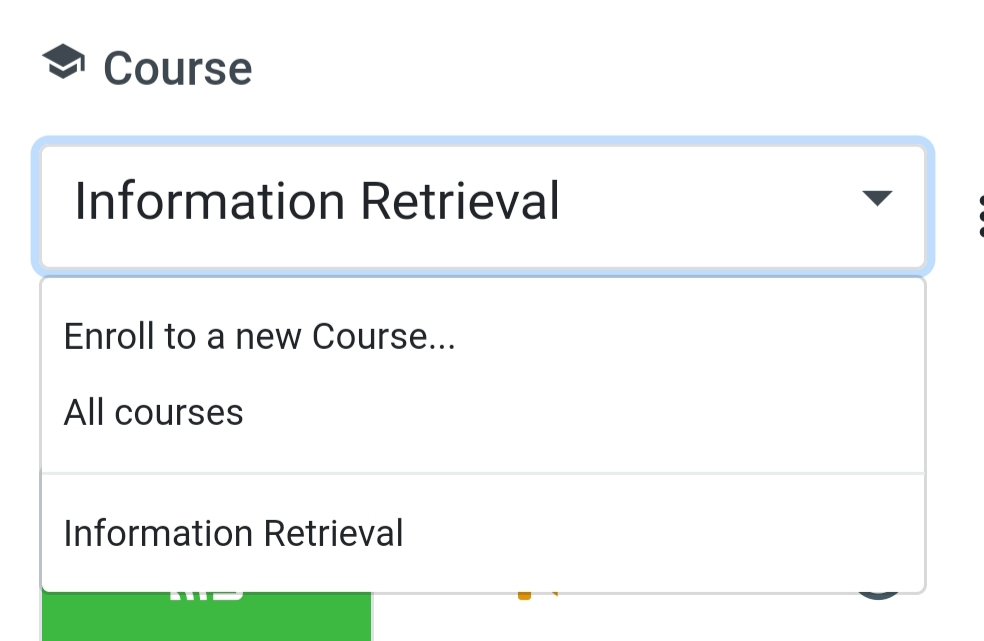
\includegraphics[width=0.95\linewidth]{screenshots/redesign/drop_down_student.jpg}
		\captionsetup{width=.8\linewidth}
		\captionsetup{format=plain}
		\caption{The \emph{Drop Down Menu} for the role \emph{Student}: The \emph{Enrollment Form} is embedded.}
		\label{fig:drop_down_student}
	\end{minipage}%
	\begin{minipage}[t]{.5\textwidth}
		\centering
		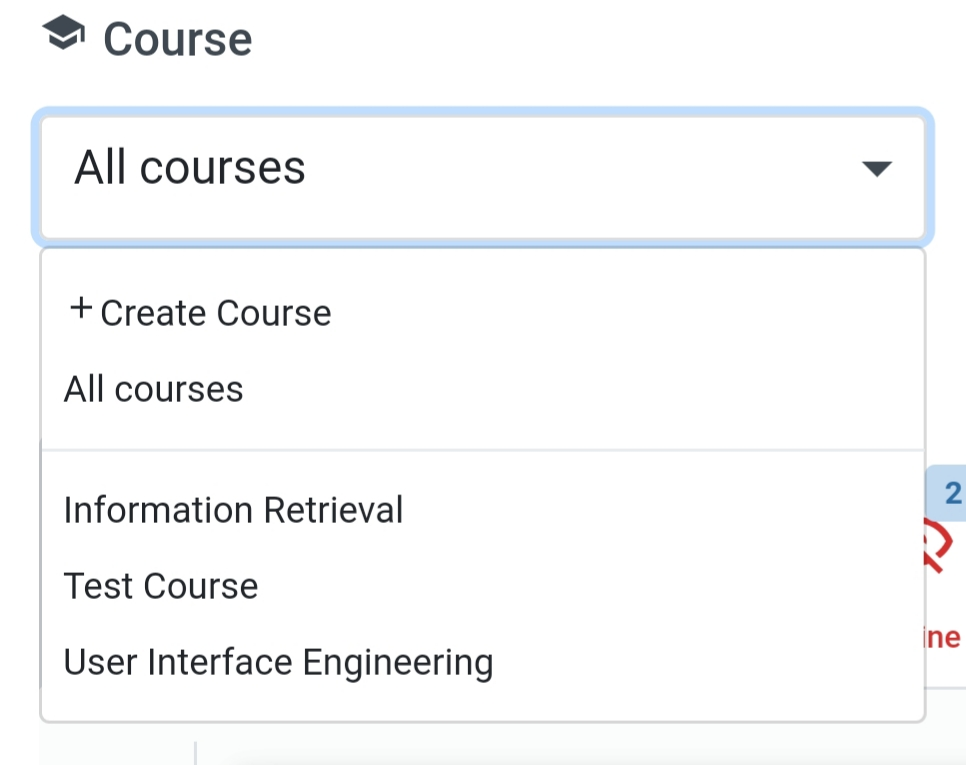
\includegraphics[width=0.95\linewidth]{screenshots/redesign/drop_down_lecturer.jpg}
		\captionsetup{width=.8\linewidth}
		\captionsetup{format=plain}
		\caption{The \emph{Drop Down Menu} for the role \emph{Lecturer}. A menu entry that allows for course creation replaces the embedded \emph{Enrollment Form}.}
		\label{fig:drop_down_lecturer}
	\end{minipage}
\end{figure}

\section{Main View}

The \emph{Main View} has undergone several revisions and does not exactly resemble the mock-ups that were shown in the previous chapter (see \Cref{figure:mainviewenhancement3}). The general layout stayed roughly the same, keeping the idea of a \emph{Drop Down Menu} and \emph{Lecture Tabs} below. But a lack of consideration for the different \emph{Roles} users can play when using AMCS made a small number of changes and considerations necessary.
\\
\\
The view consists of the \emph{Drop Down Menu} on the top that allows for course selection and \emph{Lecture Tabs} on the bottom that displays lectures sorted by their temporal context. Between the two of them, a context-sensitive \emph{Actions Menu} is displayed.
\subsection{Drop Down Menu}
Generally speaking, the \emph{Drop Down Menu} provides a coarse grain filter that allows the user to select a specific course. Doing so causes the \emph{Lecture Tabs} and their content to change accordingly.
More specifically, the \emph{Drop Down Menu} acts in a slightly different manner depending on the current user role. When using it as a \emph{Student} (see \Cref{fig:drop_down_student}), it contains all courses that said student is enrolled to. On top of that, the \emph{Enrollment Form} is embedded inside the menu, allowing the \emph{Student} to join other courses.
\\
\\
\\
In contrast, when logged in as a \emph{Lecturer} (see \Cref{fig:drop_down_lecturer}), the \emph{Drop Down Menu} contains all courses that he owns and manages. Naturally, the \emph{Enrollment Form} is omitted as the \emph{Lecturer} role does not need it.Selecting a course from the list causes an additional component to be displayed: the \emph{Actions Menu}.
\subsection{Actions Menu}
An oversight not covered by the proposals is the fact that the functionality offered by the \emph{Main View} has to change depending on the role of the user that is currently logged in. To address this issue more effectively, the \emph{Actions Menu} is introduced.
The \emph{Actions Menu} offers several buttons with different functionality derived from user roles and privileges.
The number and kind of buttons displayed in the \emph{Actions Menu} varies depending on role of the user that is currently logged in. \emph{Students} are shown the buttons for either visiting the \emph{Question Pool} or \emph{Leaving} the course altogether. In contrast, if a \emph{Lecturer} is logged in, the \emph{Action Menu} contains more options. A \emph{Lecturer} can \emph{Create a Lecture}, \emph{Edit, Export, Clone, Evaluate } or \emph{Delete} a course. Visualization and placement of the \emph{Actions Menu} is explained in the sections following.


\subsection{Lecture Tabs}
The \emph{Lecture Tabs} are displayed below the \emph{Drop Down Menu}. Each temporal context is associated with a color, label, and icon to allow for easier differentiation between them. Similar to the \emph{Actions Menu}, the concept for displaying lectures had to be adapted to comply with the semantics of different user roles.
If a \emph{Student} is logged in, the tabs \emph{Live}, \emph{Upcoming} and \emph{Past} are shown. An additional tab labeled \emph{Offline} is displayed when logged in as a \emph{Lecturer}, as \emph{Lecturers} are able to create lectures in advance and restrict access to them by changing their status to \emph{Offline}.
\\
\\
For each tab, an indicator for the number of lectures belonging to it is provided.
Tapping on one of the tabs displays the lectures in a vertical list. Instead of using paging to divide the content into shorter lists as proposed in \Cref{figure:mainviewenhancement3}, the whole list of lectures is displayed at once.
This decision was made partly because the existing code base was difficult to adapt to these criteria.

\begin{wrapfigure}{r}{0.5\textwidth}
	\vspace*{-2cm}
	\begin{center}
		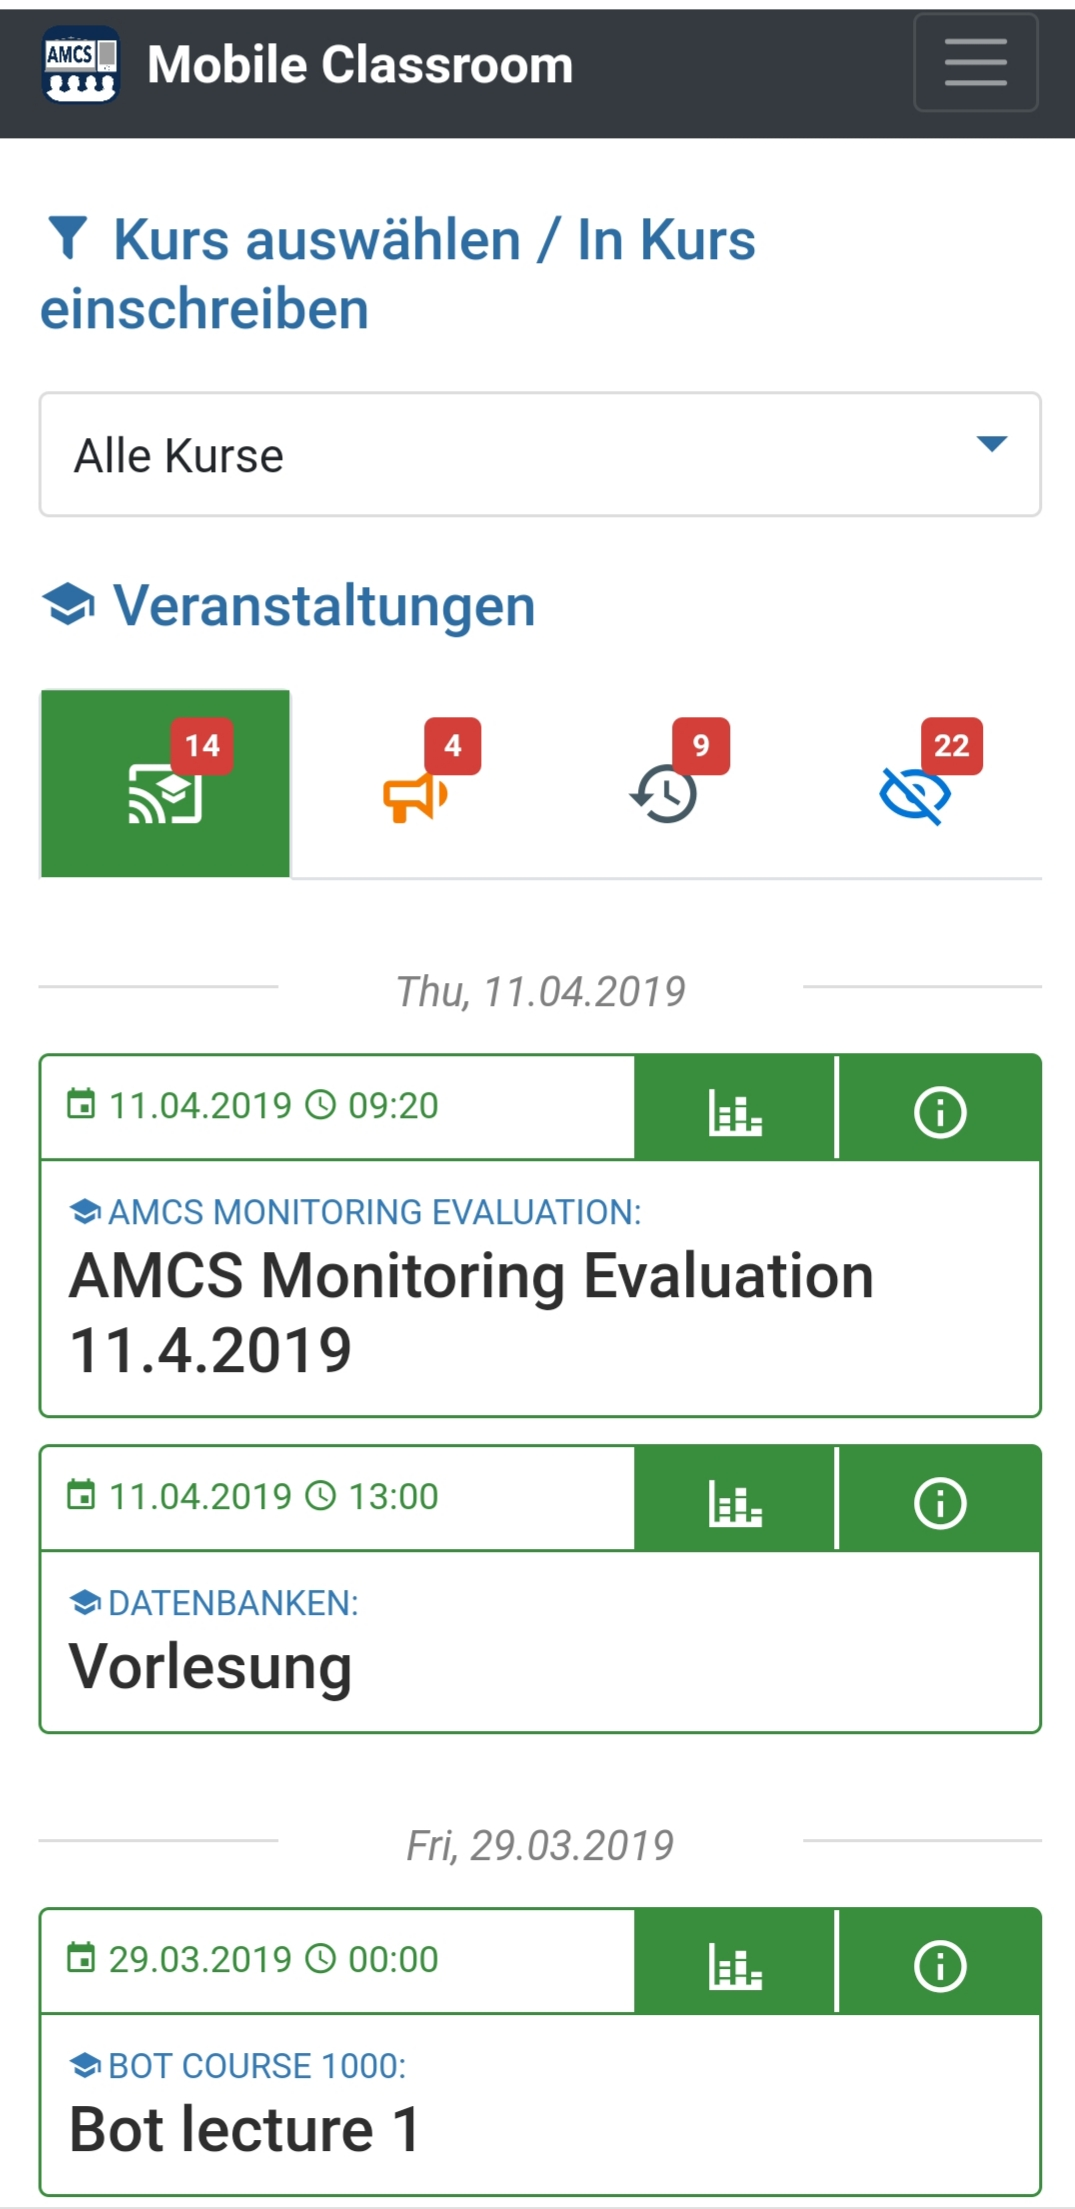
\includegraphics[width=0.48\textwidth]{screenshots/redesign/main_view_iteration_1.jpg}
	\end{center}
	\captionsetup{format=plain}
	\caption{Iteration 1 of the \emph{Main View}.}
	\label{fig:main_view:_it1}
	\vspace*{-1.5cm}
\end{wrapfigure}

\subsection{Lecture List}
The visualization of lectures underwent several different iterations before it was finalized for the evaluation. Each iteration introduced small but significant changes to the overall look and feel of the user interface.
In general, each lecture is displayed in a box colored according to the temporal context of the lecture.
The course name is displayed in a smaller font. Below that, the full title of the lecture is shown in a slightly bigger and bold font. Reading this information from top to bottom conveys the hierarchical structure of courses consisting of lectures. 

\subsubsection{Iteration 1}
Lectures are grouped by date and a visual divider between dates is introduced to emphasize and visualize this grouping (see \Cref{fig:main_view:_it1}). Each lecture is displayed in a color-coded box. On the top, the date of the lecture is displayed along with two buttons. The first button on the left will redirect to the \emph{Evaluation of Answers} functionality. 
At first, to save space, only the course name and the lecture title are shown. The description of the lecture below is deemed not as important and is therefore retracted per default. The second button on the top right can be used to unveil the lecture description.
The \emph{Actions Menu} as such was not part of this iteration yet.

\paragraph{Problems}
The date divider does not eliminate the redundancy introduced by displaying the date of each lecture individually.
Furthermore, the design of the two buttons on the top right might be problematic. For once, it can be difficult to identify these two elements with their placement and lack of textual labels as pressable buttons. While collecting intermediate feedback from the AMCS group, people tended to say that they struggle with identifying the meaning of the iconography used. 

\subsubsection{Iteration 2}
The second iteration addresses the problems described above partly (see \Cref{fig:main_view:_it2}). Most notably, the \emph{Lecture List} resembles more a calendar or a student schedule in its overall design. The layout is divided into two columns: The left column displays the current date, whereas the right column contains the list of courses associated with the date. Essentially, instead of displaying the date for each lecture, this information is extracted to the left column. Now, only the time and duration are displayed at the top for each lecture separately. The description remains retractable.
\begin{wrapfigure}{l}{0.5\textwidth}
	\vspace*{-0.5cm}
	\begin{center}
		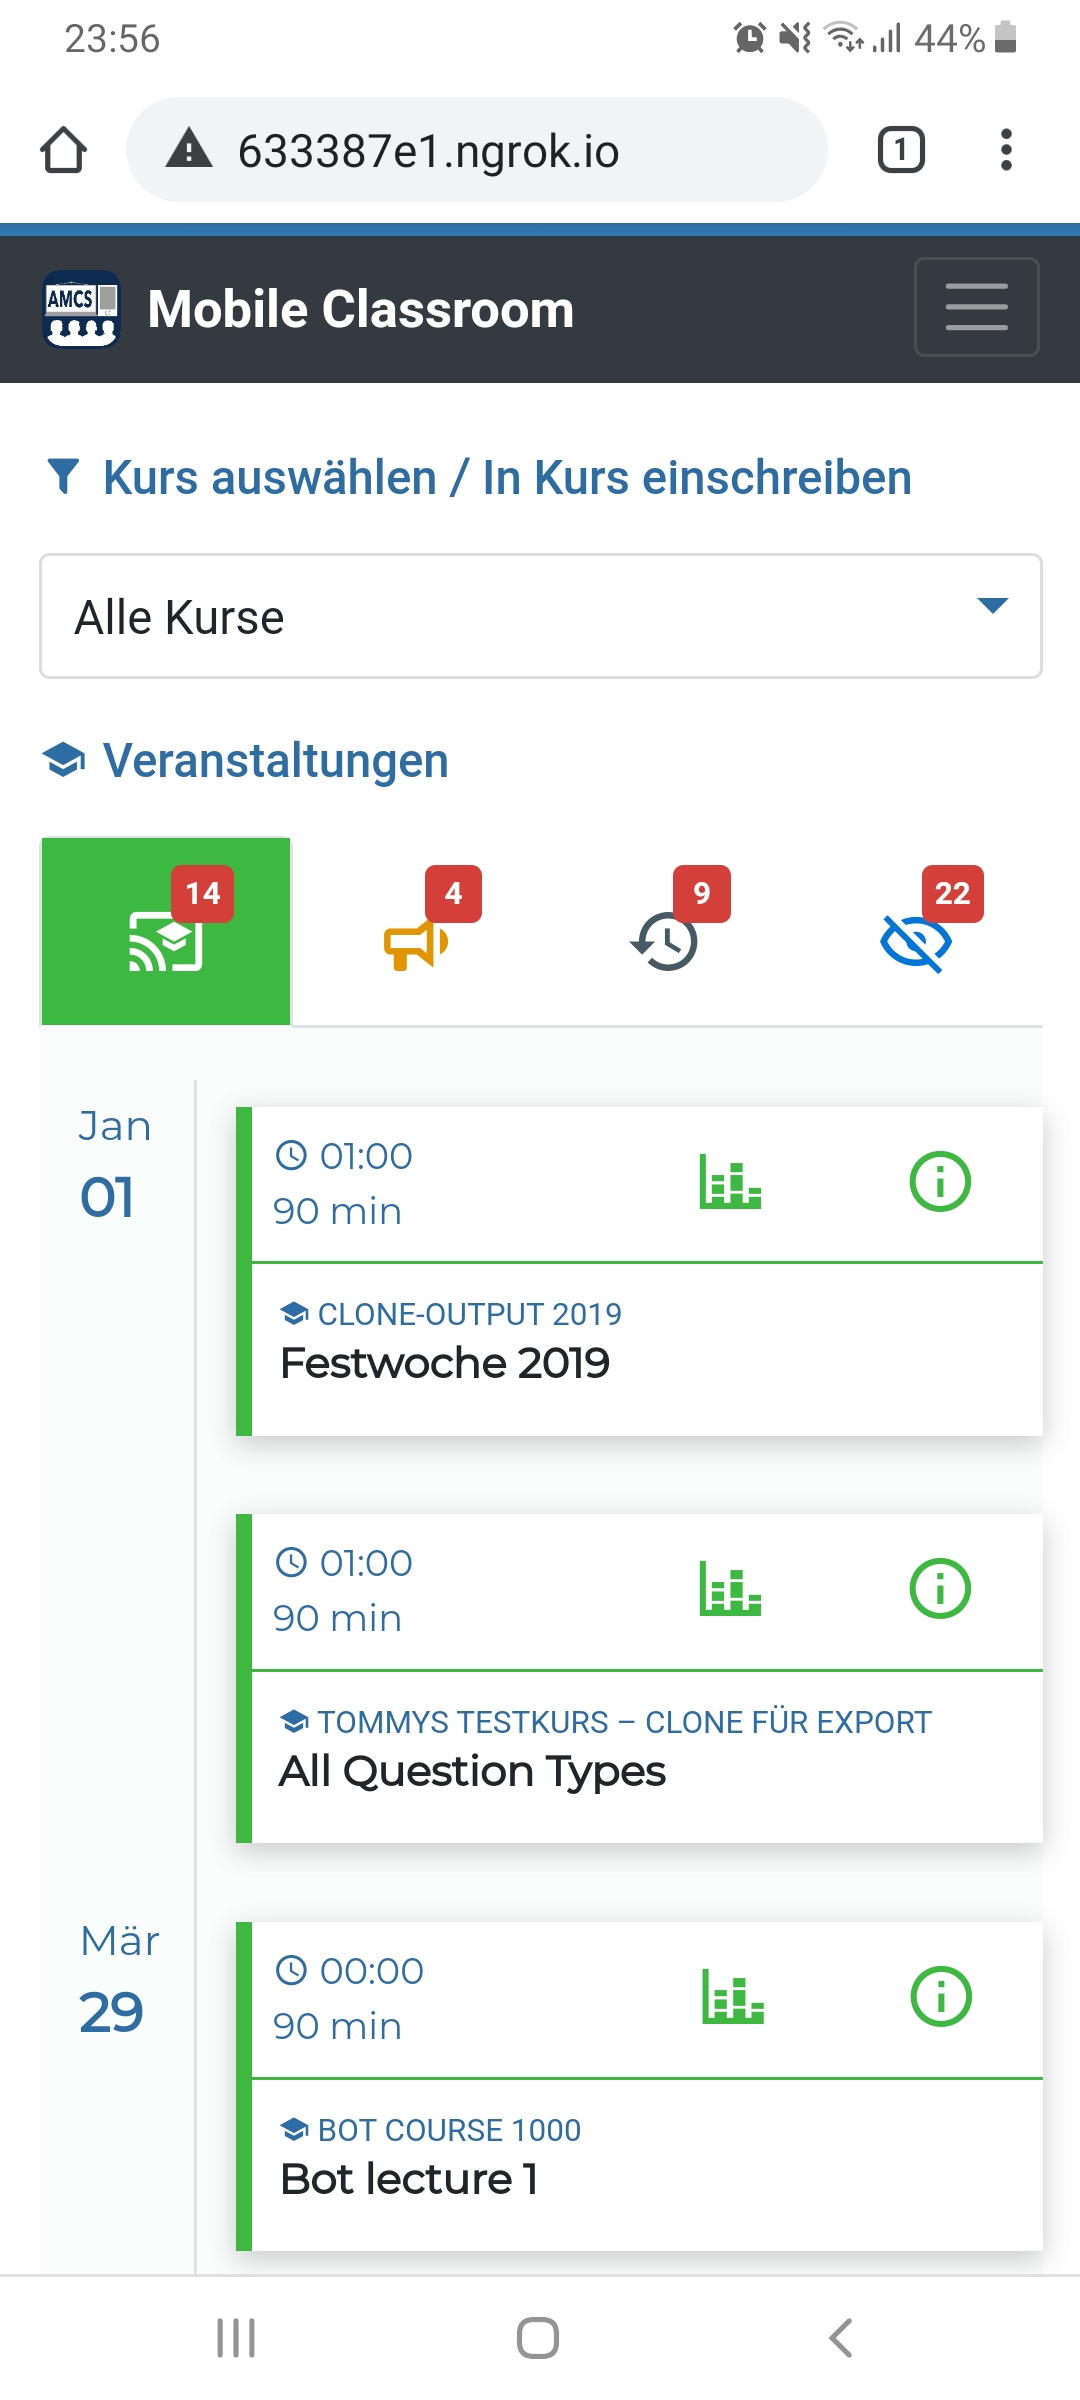
\includegraphics[width=0.48\textwidth]{screenshots/redesign/main_view_iteration_2.jpg}
	\end{center}
	\captionsetup{format=plain}
	\caption{Iteration 2 of the \emph{Main View}. Four tabs are displayed when logged in as a \emph{Lecturer}. From left to right: \emph{Live, Upcoming, Past, Offline}.}
	\label{fig:main_view:_it2}
	\vspace*{-1.5cm}
\end{wrapfigure}
The buttons on the top of each lecture have the colors of their background and icon inverted, but they essentially remained the same.
Furthermore, each lecture box is given a drop shadow to indicate that the area is pressable. Pressing anywhere on this \emph{card-like} box will redirect students to the \emph{Poll View}, whereas lecturers will arrive at the \emph{Course Dashboard}.

\paragraph{Problems}
Similar to the ambiguity of the top buttons of each lecture that remains in this iteration, every \emph{tab} is suffering from the same problem. According to feedback from the AMCS group, the used iconography alone fails to convey which temporal context each tab is representing.

\subsubsection{Iteration 3}
Some issues regarding the \emph{Lecture List} are fixed in this iteration.
To clarify the meaning of each \emph{tab}, a textual label is added. 
The colors of each tab are adjusted slightly to be more easy on the eyes (see \Cref{fig:main_view_tab_labels}). Furthermore, improvements to the \emph{Lecture Box} design are made (see \Cref{fig:main_view_lecture_box_buttons}). The time and duration of each lecture are displayed in one line next to each other. The two buttons previously discussed are moved to the bottom. They are expanded to take most of the width of the lecture box. The icons remain the same but they are reduced in size and pushed to the left.
A textual label in the center of each button now describes its purpose.
\\
\\
This iteration also includes the introduction of the aforementioned \emph{Actions Menu}. It consists of a vertical list of buttons and remains completely hidden if the entry \emph{All courses} is selected from the \emph{Drop Down Menu}. This design hopes to remove unnecessary clutter by displaying these buttons only when needed.

\begin{figure}
	\centering
	\begin{minipage}[t]{.5\textwidth}
		\centering
		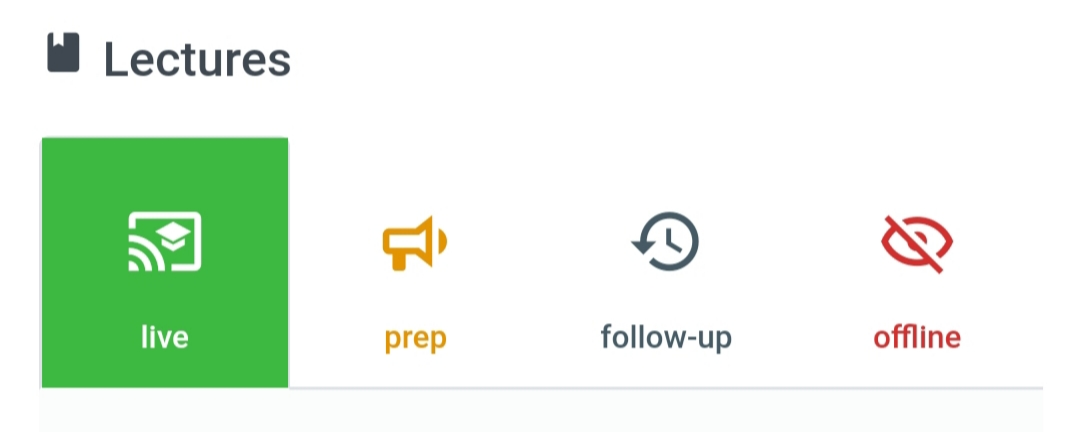
\includegraphics[width=0.95\linewidth]{screenshots/redesign/lecture_tab_labels.jpg}
		\captionsetup{width=.8\linewidth}
		\captionsetup{format=plain}
		\caption{Improved \emph{Lecture Tabs} of \emph{Iteration 3} with textual labels. The \emph{Offline} tab is displayed only to \emph{Lecturers}.}
		\label{fig:main_view_tab_labels}
	\end{minipage}%
	\begin{minipage}[t]{.5\textwidth}
		\centering
		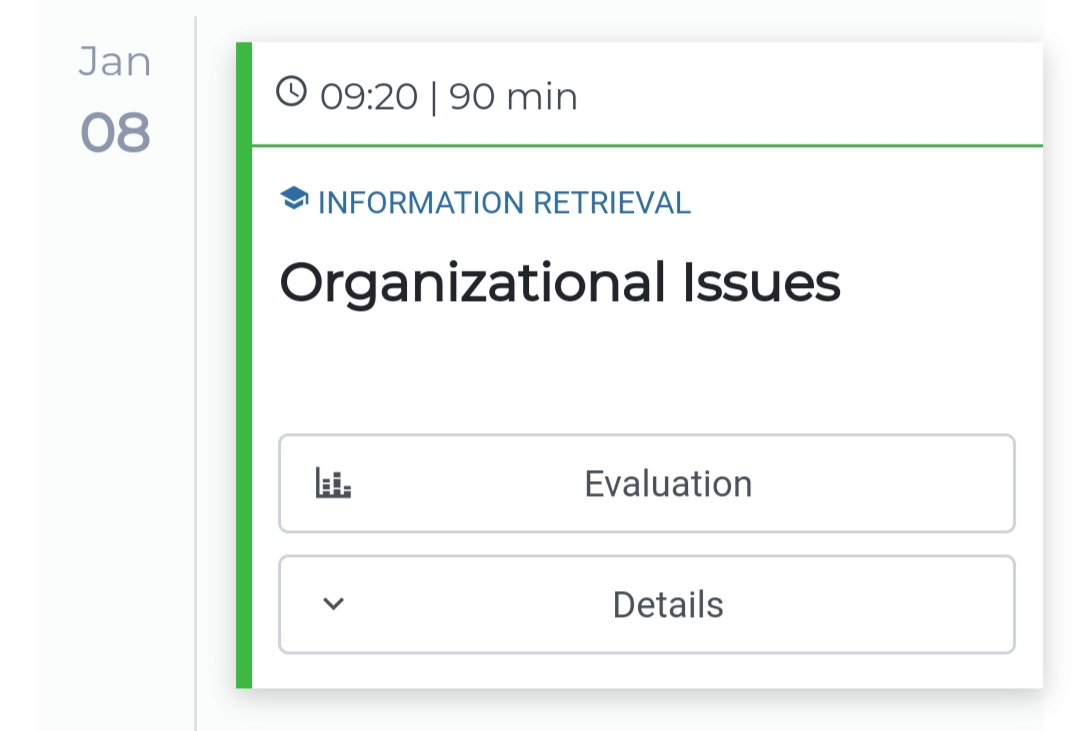
\includegraphics[width=0.95\linewidth]{screenshots/redesign/main_view_it3_lecture_box.jpg}
		\captionsetup{width=.8\linewidth}
		\captionsetup{format=plain}
		\caption{Improved \emph{Lecture Box} of \emph{Iteration 3}. The two buttons, previously at the top and unlabeled, are now located at the bottom.}
		\label{fig:main_view_lecture_box_buttons}
	\end{minipage}
\end{figure}
\paragraph{Problems}
The introduction of the \emph{Actions Menu} raises new problems. The buttons are organized in a vertical list that pushes all following content further down the page. This problem is essentially identical to the issue that occurred with the original \emph{Burger Menu}. After pressing one of the buttons of the \emph{Actions Menu}, content below might change. However, in some cases, because the menu itself stays in place, these updates of the user interface below might happen completely off screen. Therefore, selecting some of the buttons could feel to the user like an idempotent operation.

\subsection{Iteration 4}
\begin{wrapfigure}{r}{0.55\textwidth}
	\vspace*{-1cm}
	\begin{center}
		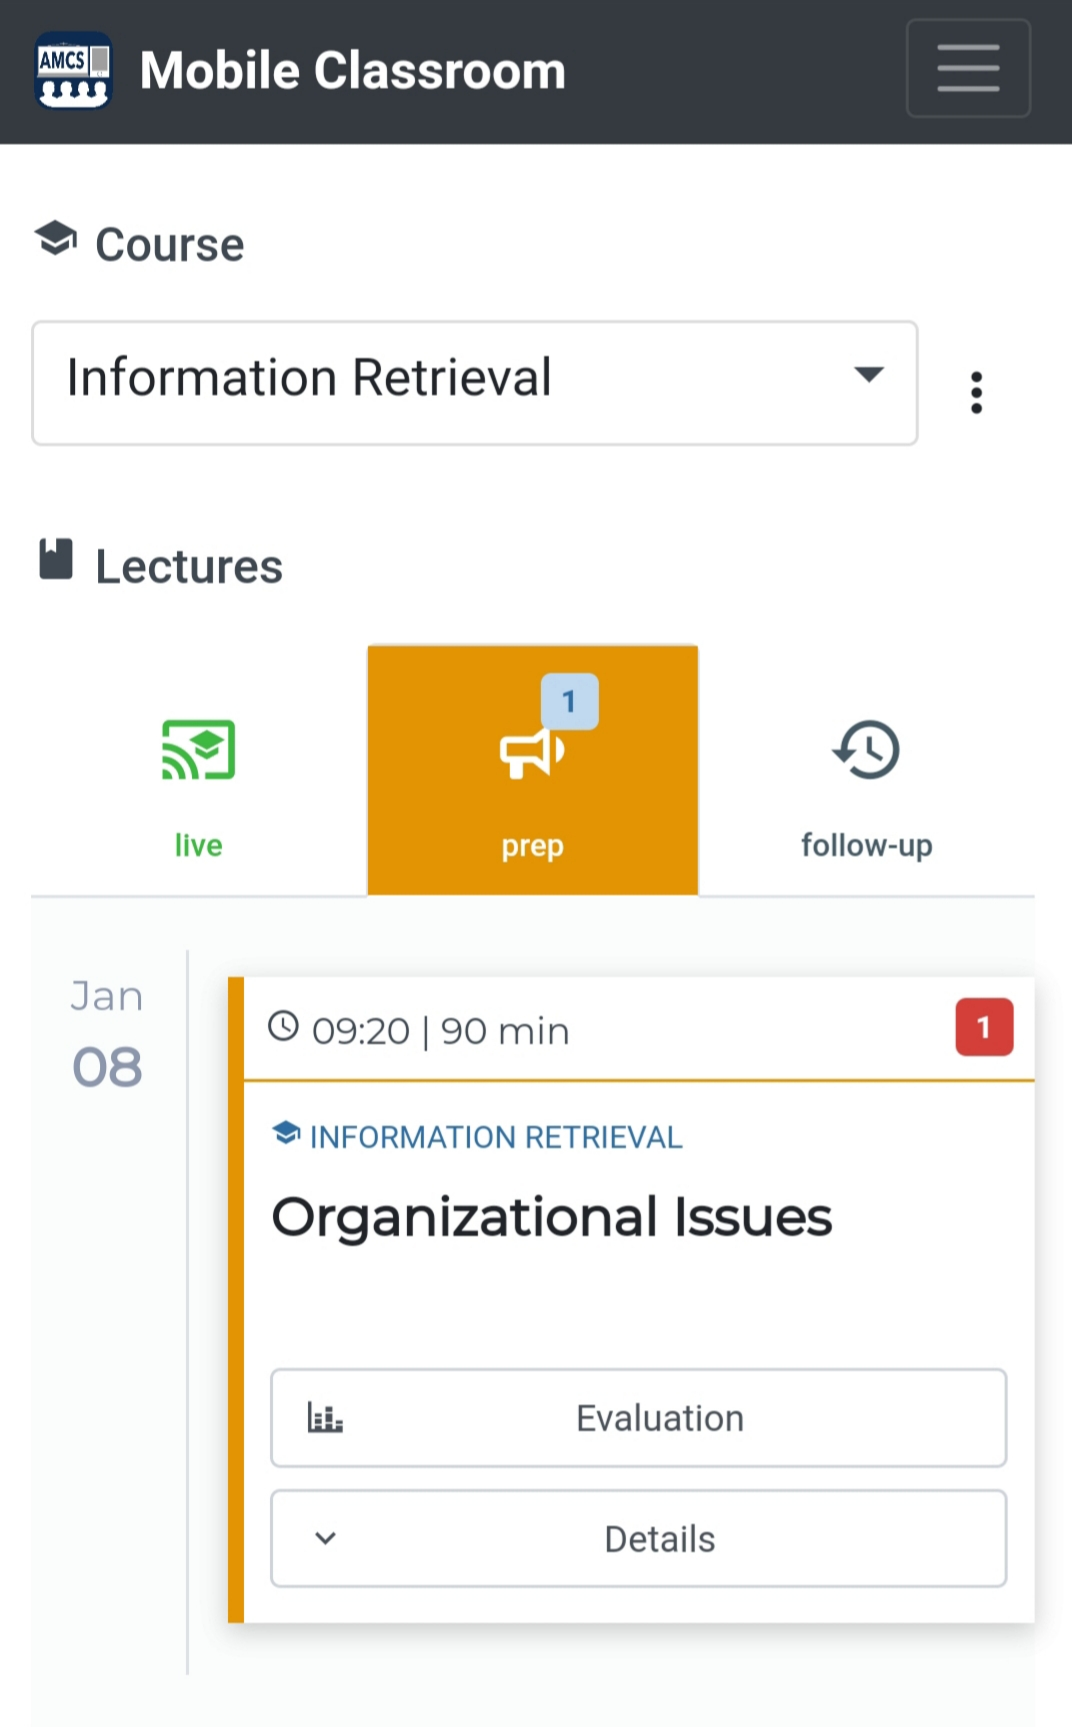
\includegraphics[width=0.48\textwidth]{screenshots/redesign/main_view_iteration_4.jpg}
	\end{center}
	\captionsetup{format=plain}
	\caption{\emph{Iteration 4}: The \emph{Action Menu} is now accessed by pressing the \emph{Three-Dots-Button} next to the \emph{Drop Down Menu}. Furthermore, an indicator for unanswered polls is added to the \emph{Lecture Box}.}
	\label{fig:main_view_iteration_4}
\end{wrapfigure}

\begin{figure}
	\vspace{1cm}
	\centering
	\begin{minipage}[t]{.5\textwidth}
		\centering
		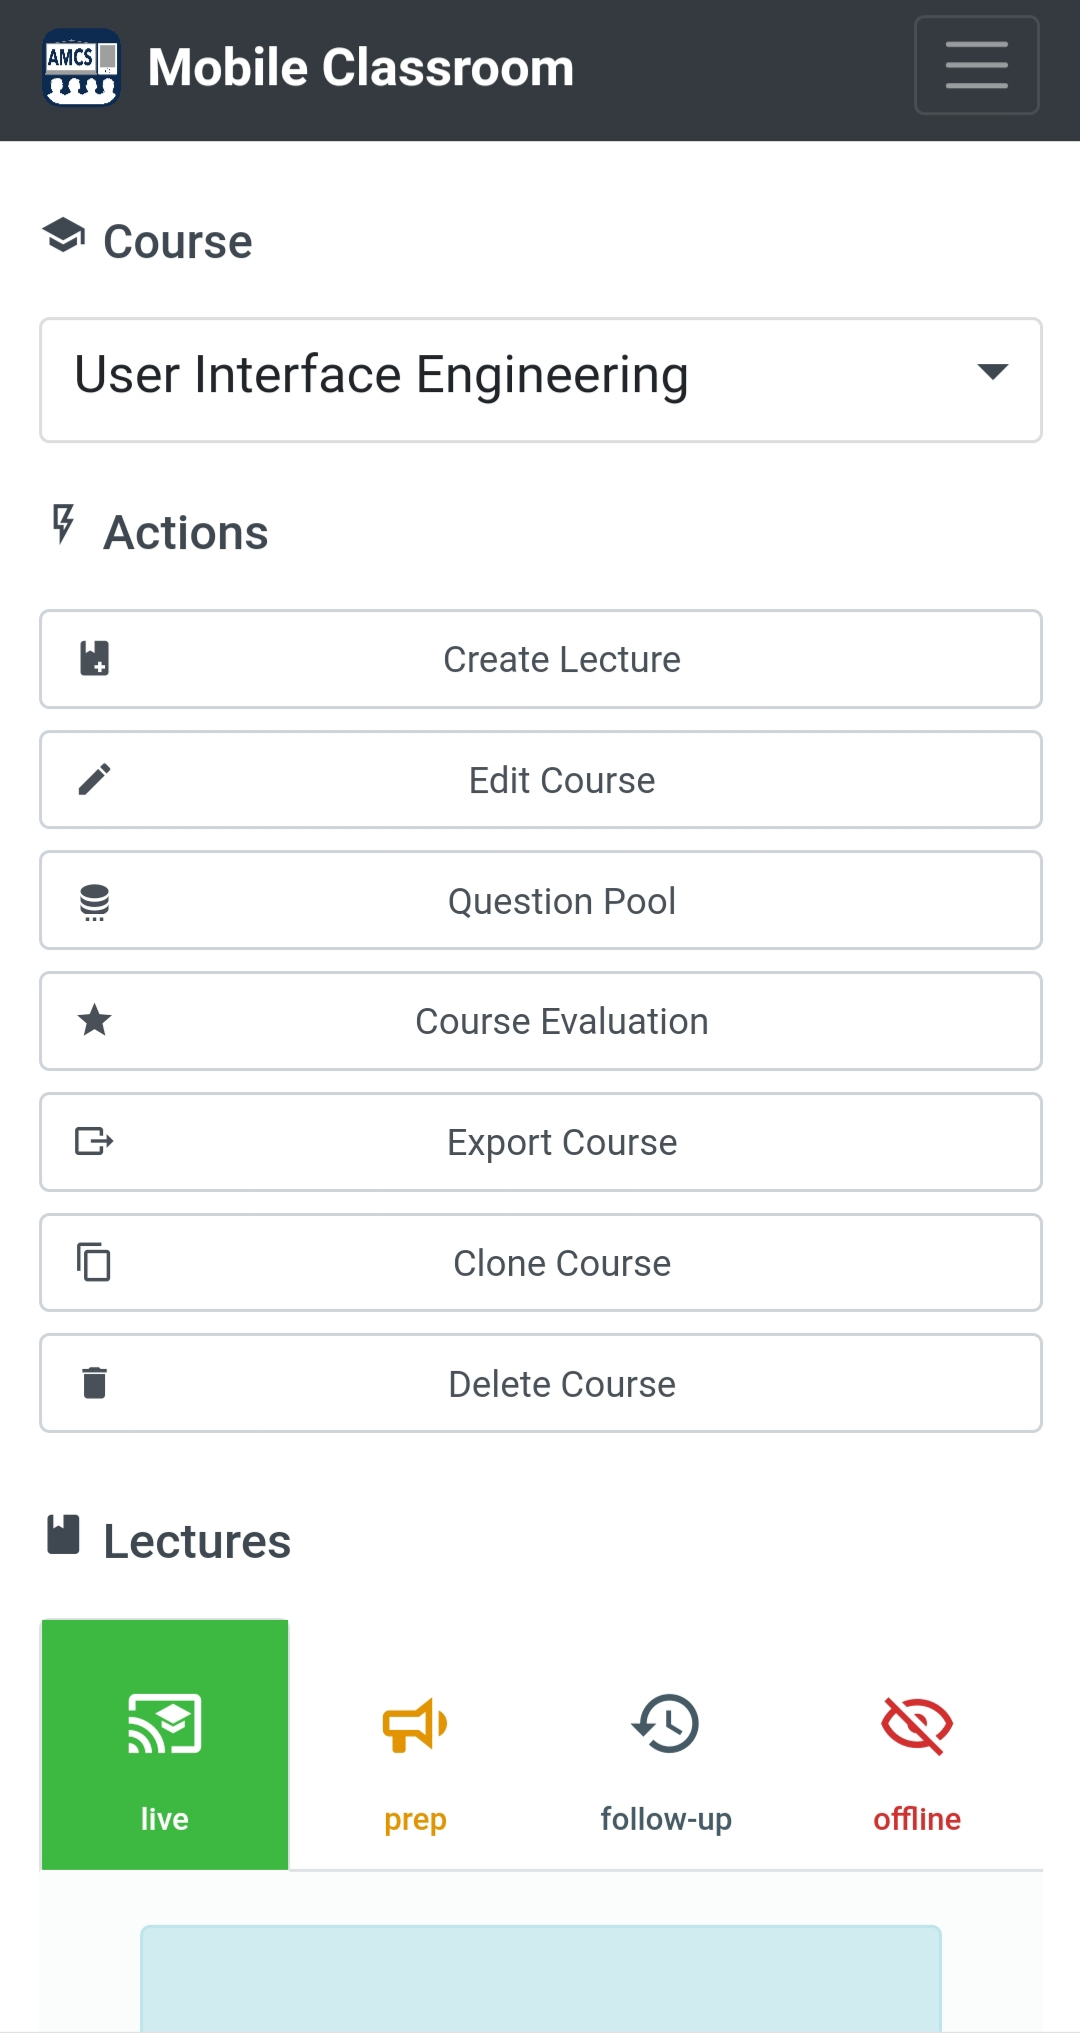
\includegraphics[width=0.95\linewidth]{screenshots/redesign/problem_main_view_course_actions.jpg}
		\captionsetup{width=.8\linewidth}
		\captionsetup{format=plain}
		\caption{\emph{Actions Menu for Lecturer} in \emph{Iteration 3}: The \emph{Lecture Tabs} and any other content below is always displaced by the long list of buttons, because it never disappears. }
		\label{fig:main_view_course_options_bad}
	\end{minipage}%
	\begin{minipage}[t]{.5\textwidth}
		\centering
		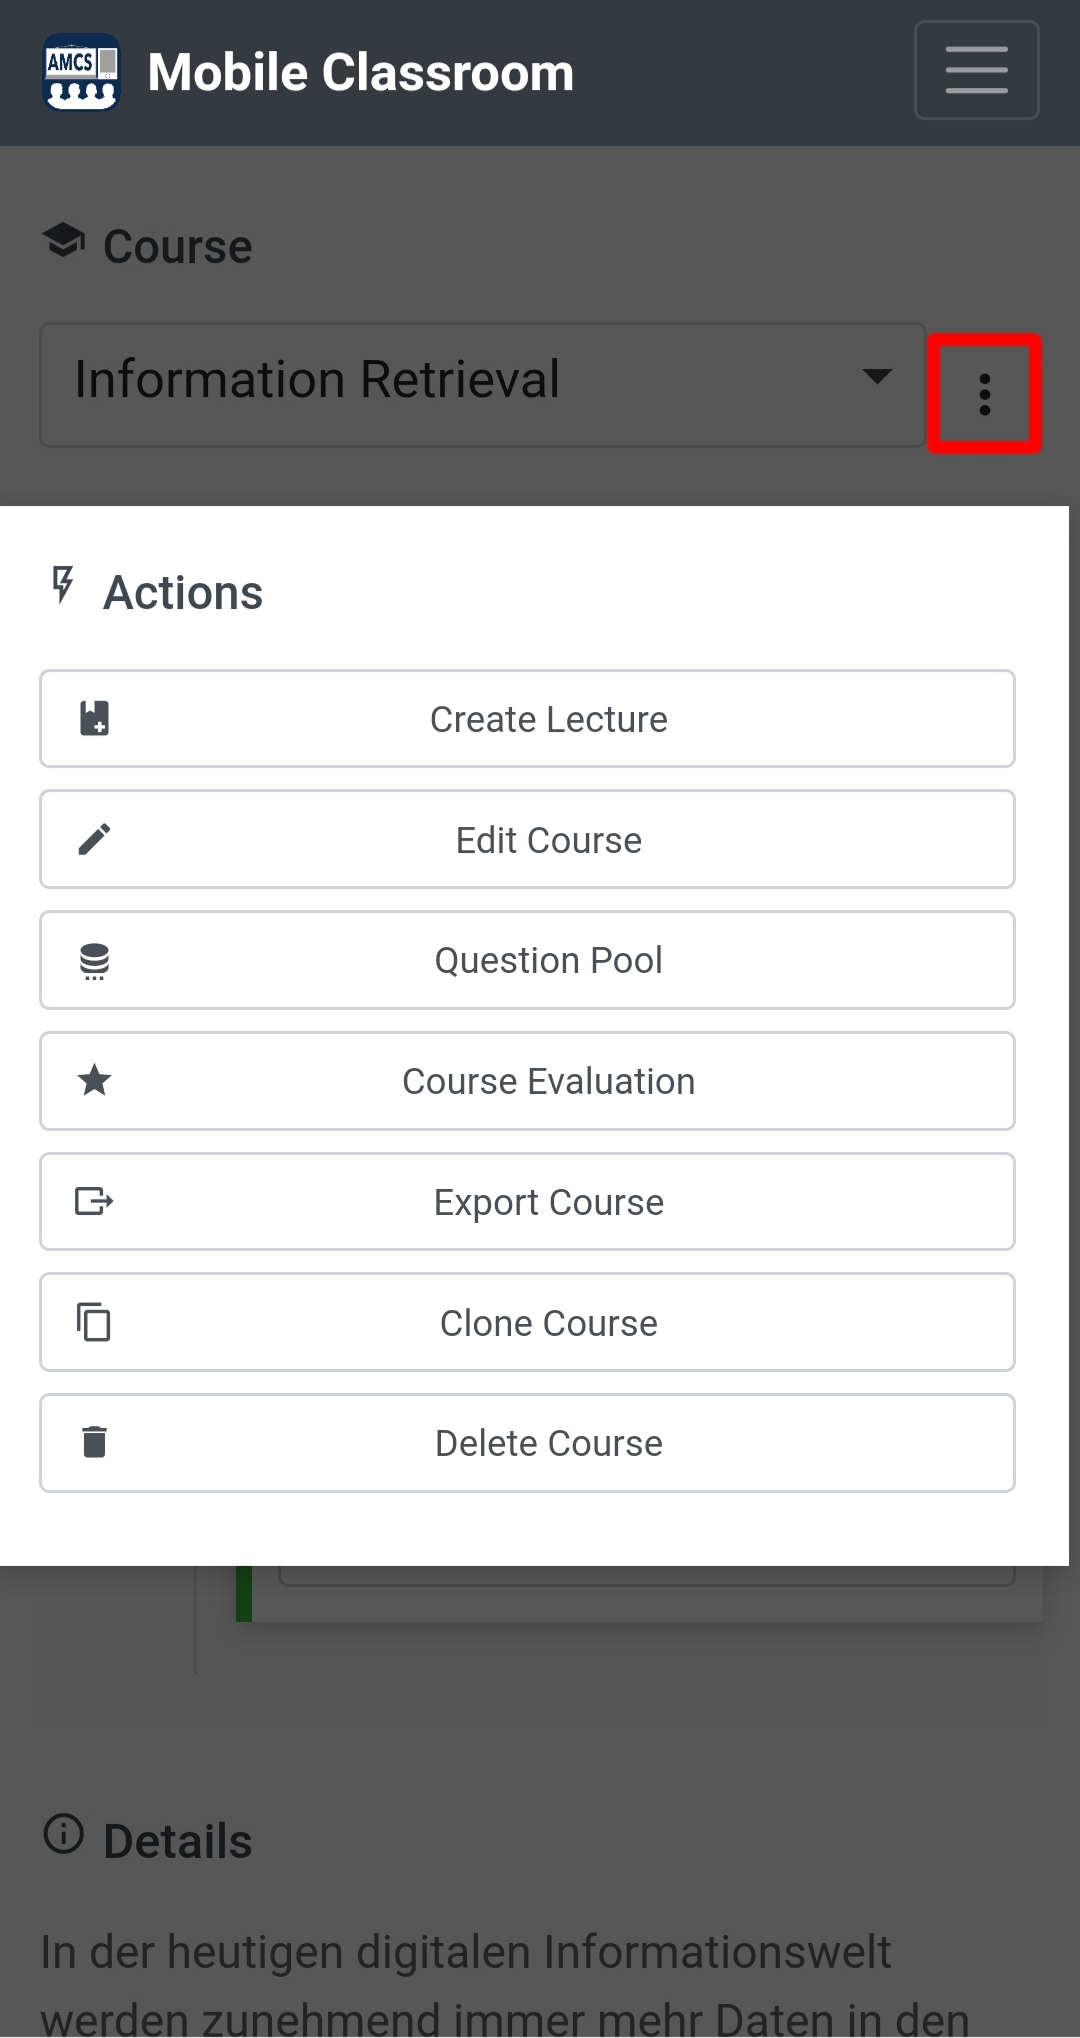
\includegraphics[width=0.95\linewidth]{screenshots/redesign/main_view_iteration_4_actions.jpg}
		\captionsetup{width=.8\linewidth}
		\captionsetup{format=plain}
		\caption{Improved \emph{Actions Menu} of \emph{Iteration 4}: An extra button denoted by three dots (in the red square) toggles an overlay that contains the \emph{Actions Menu}. It closes once a selection is made, preventing displacement of the content below.}
		\label{fig:main_view_course_options_good}
	\end{minipage}
\end{figure}

\emph{Iteration 4} represents the last incremental update to the \emph{Main View} (see \Cref{fig:main_view_iteration_4}).
Most prominently, the  \emph{Action Menu} is now hidden per default. 
A new button next to the \emph{Drop Down Menu} suggests additional options that concern the selected course. Tapping this button shows the \emph{Action Menu} (see \Cref{fig:main_view_course_options_good}). Selecting one of the options from the \emph{Actions Menu} causes it to close and update the view below accordingly.
Furthermore, changes to the \emph{Lecture Tabs} are made. The \emph{Notification Bubbles} are changed slightly in style. They now serve as an absolute counter for the number of elements inside a tab.
Besides this change, a \emph{Notification Bubble} is displayed for each \emph{Lecture Box}, indicating new and unanswered questions for a given lecture. 
\section{Navigation}
As proposed earlier in \Cref{chapter:concept}, the \emph{Burger Menu} was slimmed down considerably. A logged in user can only find the menu entries \emph{Edit account}, \emph{How it works} and \emph{Logout} (see \Cref{fig:navigation}).
The \emph{Question Pool} and \emph{Evaluation of Answers} is moved to the respective lectures in the \emph{Main View}. Apart from these changes, the \emph{Burger Menu} stayed the same. Content below now has a higher chance to stay inside the visible viewport.
\begin{wrapfigure}{r}{0.5\textwidth}
	\vspace*{-4cm}
	\begin{center}
		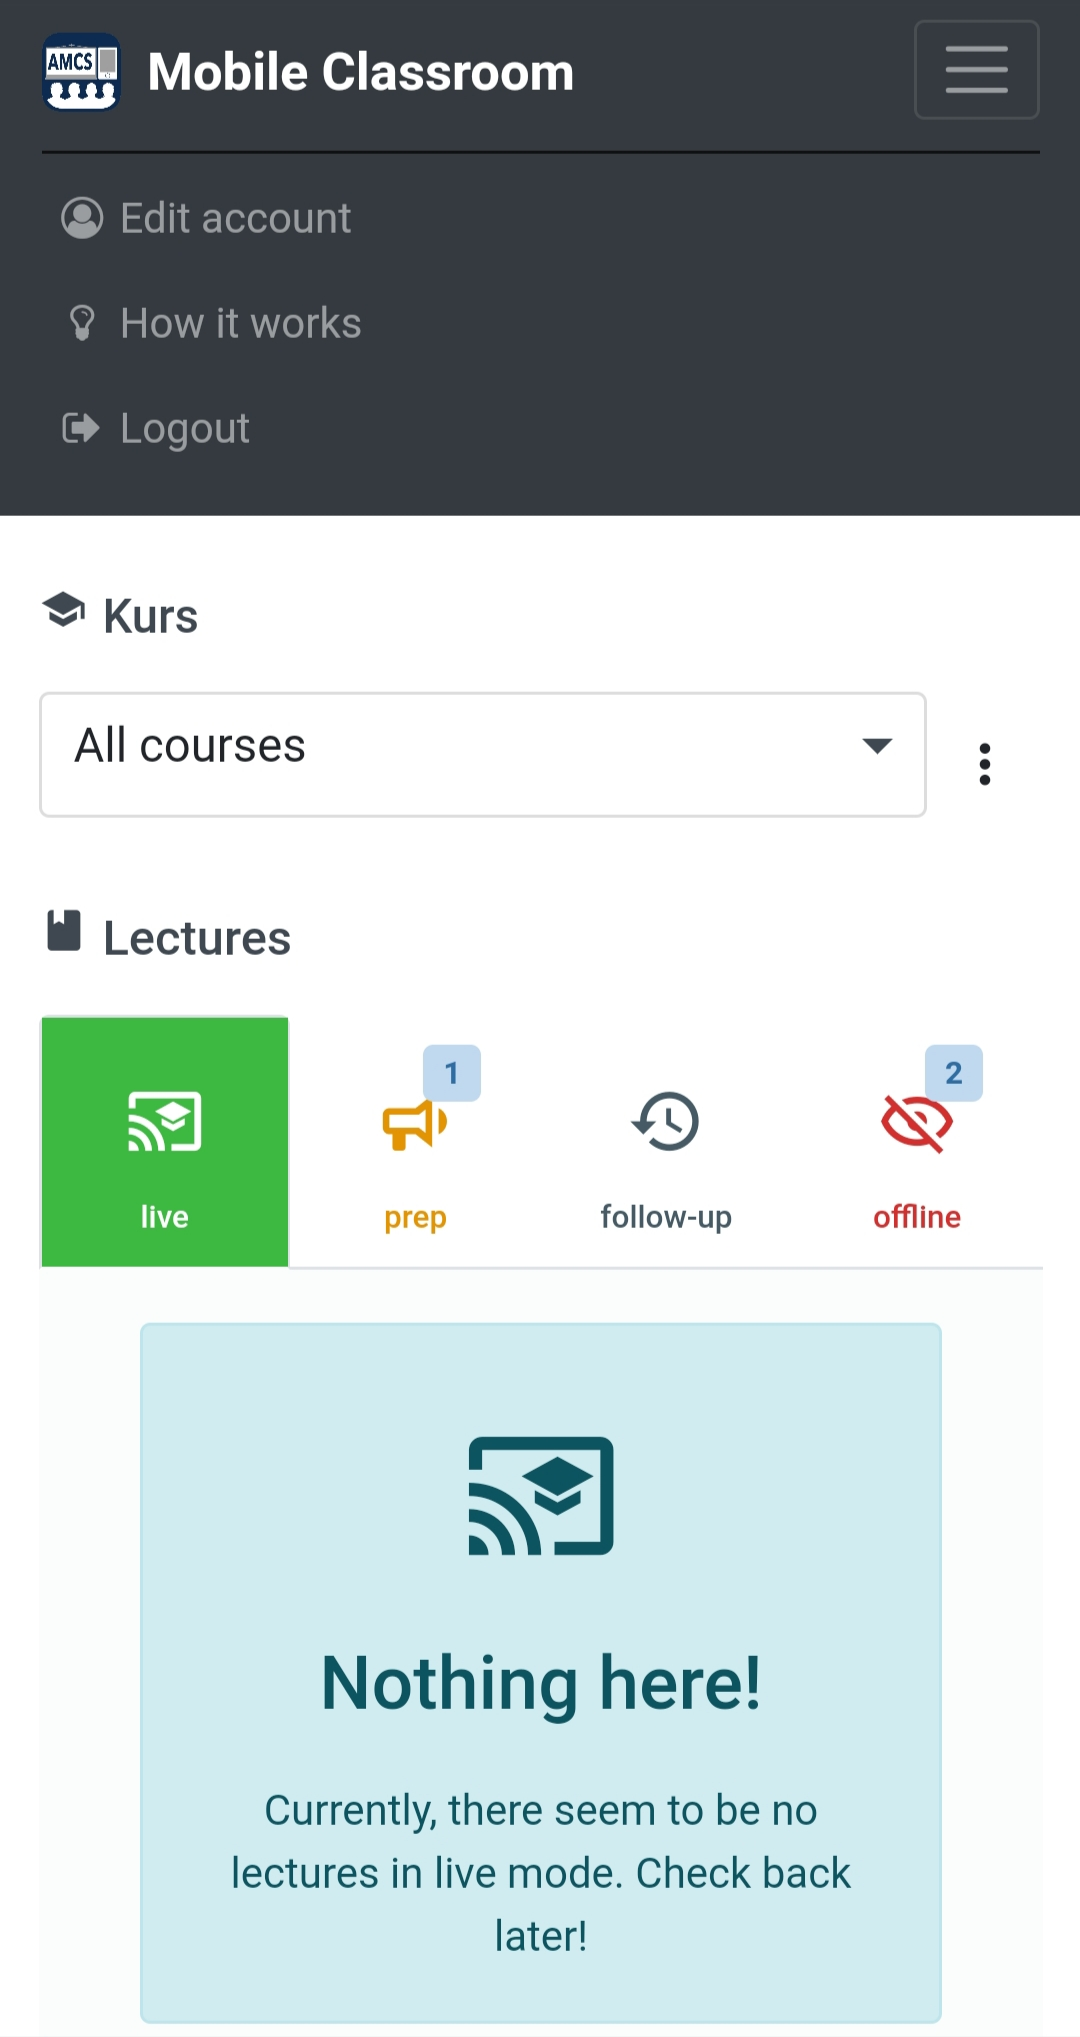
\includegraphics[width=0.48\textwidth]{screenshots/redesign/navigation_new.jpg}
	\end{center}
	\captionsetup{format=plain}
	\caption{\emph{Iteration 4}: The \emph{Burger Menu} displaces the content that follows in a significantly reduced magnitude.}
	\label{fig:navigation}
\end{wrapfigure}
\section{Poll View}
The \emph{Poll View} is implemented closer to the proposals made in \Cref{chapter:redesignstrategy} than the \emph{Main View} previously described. Nevertheless, several changes had to be made to account for the hard to extend codebase.    

\subsection{Layout}
The layout of the \emph{Poll View} overall stayed close to the proposals in \Cref{section:con:problems:pollview} (see \Cref{fig:pollview}). An exception is the \emph{Back Button} that was added at the top left. When pressed, it returns the user to the \emph{Main View}. Similar to the \emph{Lecture Boxes} of the \emph{Main View}, first the course name is displayed, followed by the lecture name in a bigger, uppercase font. 
As tabs are already used by the \emph{Main View}, a reusable \emph{Tab Component} was implemented to avoid duplicate code in the already complicated codebase. The \emph{Poll View} uses an instance of the component. Each poll type has a tab designated to it, complete with \emph{Notification Bubbles} showing the remainder of unanswered questions for each category respectively. To be more precise, the \emph{Slide Polls} are displayed in the \emph{Slide} tab and the \emph{Course Polls} reside in the \emph{Course} tab.
However, the \emph{Preparation-, Lecture-, and Post-Processing-Polls} are all located in the \emph{Lecture Tab}. The content that is displayed in this tab therefore directly depends on the state of the lecture.

\subsection{State updates}
The implementation behaves like the existing system in the same manner that lecture state updates or the answering of the question cause the view to update accordingly. This is achieved by leveraging the existing code that relies on a \emph{WebSocket} connection. No manual polling via a refresh by the user is required for the view to stay up to date.

\subsection{Navigation between Questions}
As described in \Cref{section:con:proposals:pollview}, the \emph{Poll View} features the \emph{Navigation Bar}, albeit slightly modified. Between the buttons for navigating \emph{forward} and \emph{backward}, each question is represented by a clickable circle. 
\begin{wrapfigure}{l}{0.5\textwidth}
	\vspace*{-0.5cm}
	\begin{center}
		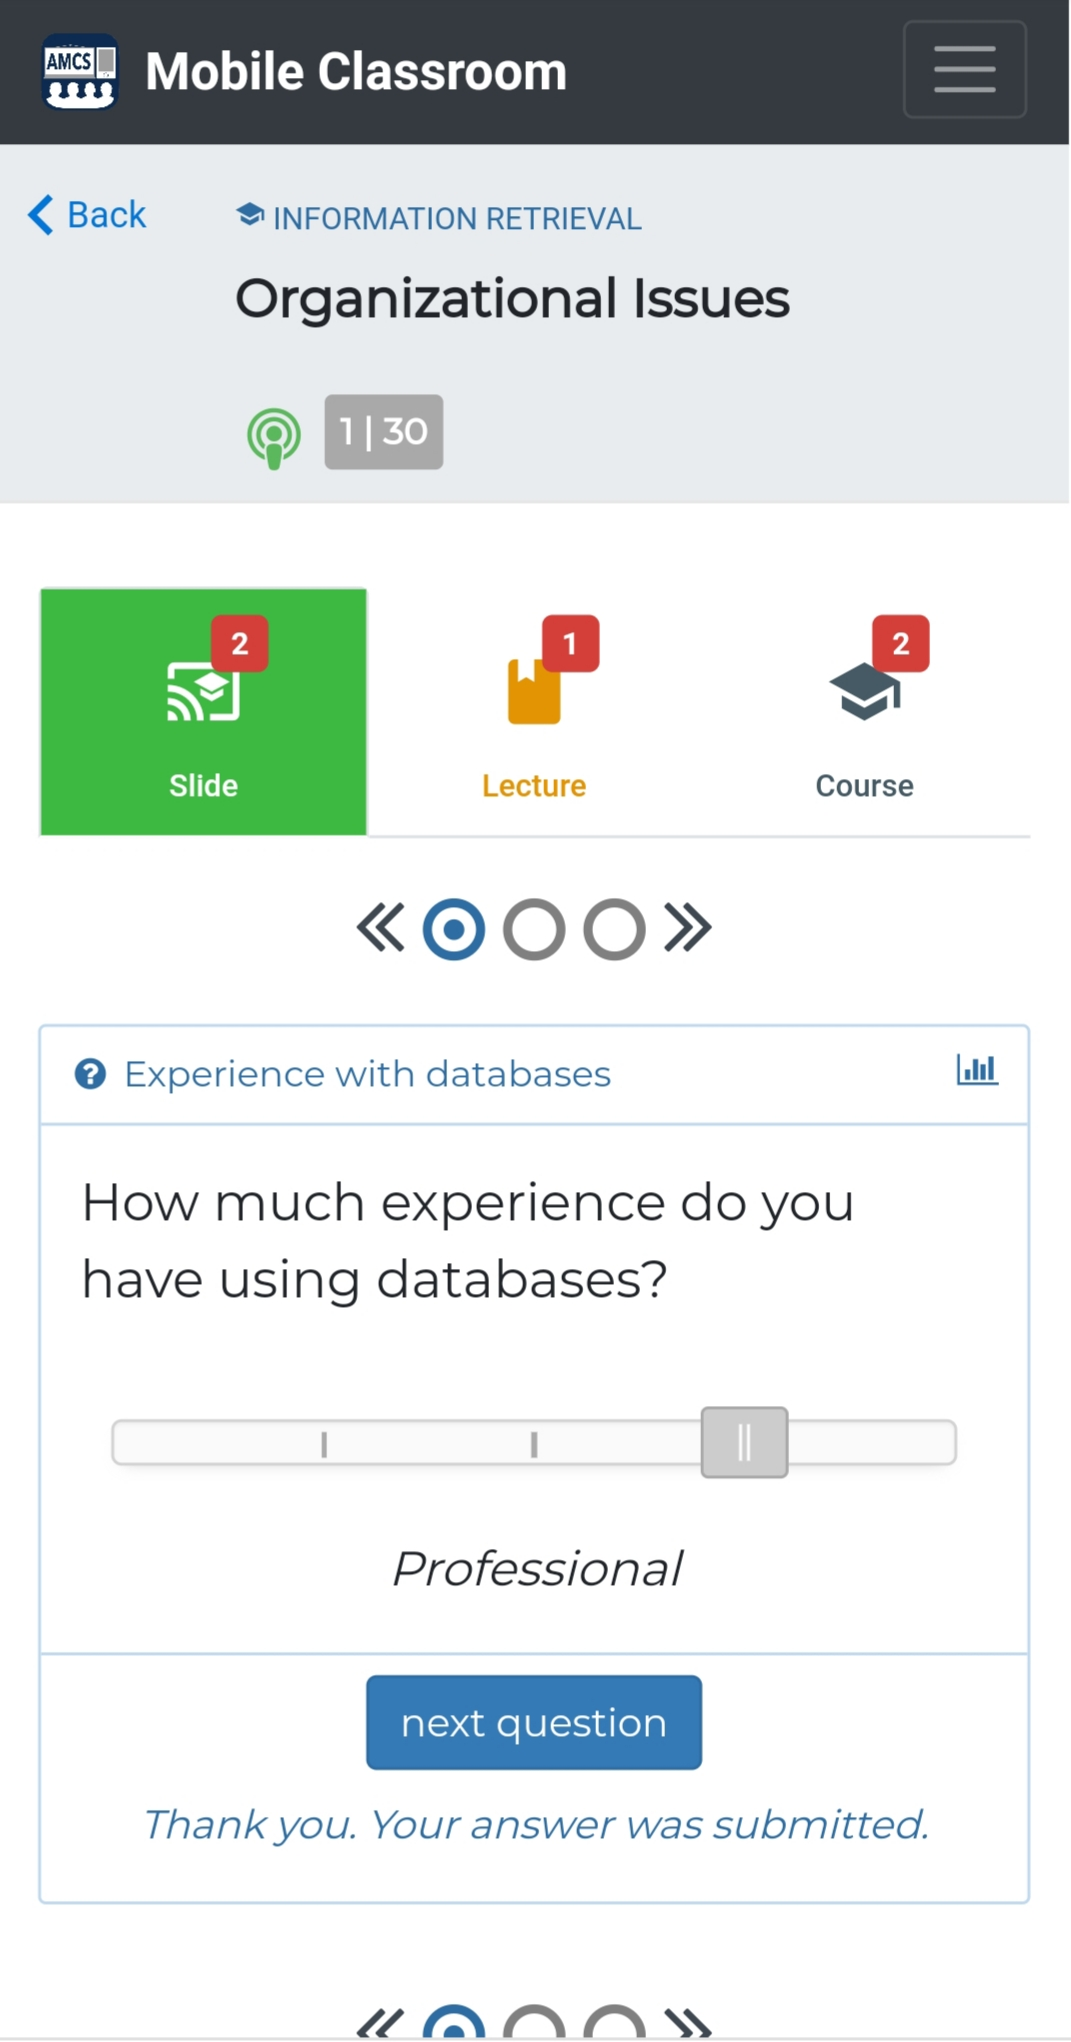
\includegraphics[width=0.48\textwidth]{screenshots/redesign/poll_view_next_question}
	\end{center}
	\captionsetup{format=plain}
	\caption{The improved \emph{Poll View} using tabs to separate polls, the \emph{Navigation Bar} and the \emph{Previous- / Next Question} buttons to ease navigation.}
	\label{fig:pollview}
\end{wrapfigure}
The current question is highlighted visually by usage of a different, blue icon.
To ease navigation even further, the \emph{Navigation Bar} is displayed a second time below the question. After answering a question, a button for advancing to the next question is shown (if a next question does exist).
\subsection{Rendering of Questions}
The existing implementations for each question type were adapted to be visually more appealing. The colors used in the prototype differ significantly from the design proposed in \Cref{figure:pollviewenhanvement2}. Most notably, the font size of the question is increased significantly to improve readability. To avoid collision with the established design of the \emph{Main View}, background colors were adjusted to be mostly white instead of a solid blue. Border colors remain in the corporate design of AMCS. 

\subsection{Problems}
Not all features were implemented, as problems occurred during development. For example, due to time constraints the feature that allows the \emph{Navigation Bar} indicates the correctness for a given answer through respective iconography was not implemented. The \emph{Next Question}-Button is only displayed, if a next question exists. Furthermore, the prototype implementation is not sophisticated enough to offer a button that allows to jump to the closest unanswered question nearby.